
\subsection*{Validation des capacités dynamiques du système de déploiement}


On s'intéresse ici au système de déploiement du sous-système SEIS. Il est basé sur un instrument hybride composé :
\begin{itemize}
\item d'un système de déploiement (DPL);
\item d'une sphère (SEIS) comportant trois capteurs sismiques à très larges bandes et leurs capteurs de
température;
\item d'une boîte électronique d'acquisition dont la structure est donnée par le diagramme de
définition des blocs. 
\end{itemize}

\begin{figure}[!h]
\centering
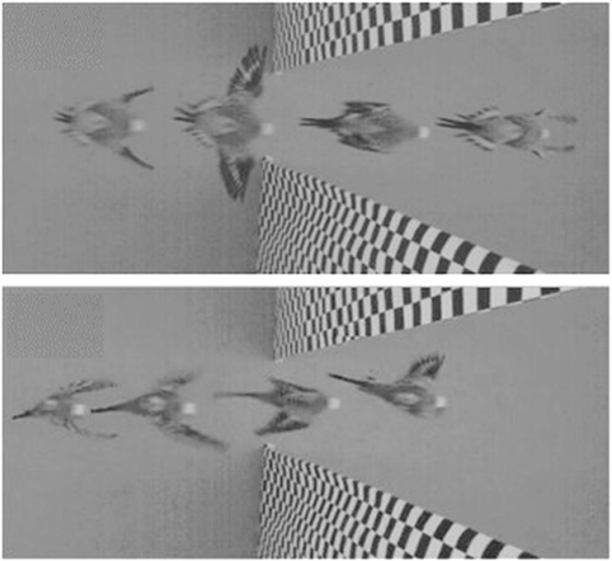
\includegraphics[width=5cm]{fig_01.png}
\caption{Sous-système SEIS \label{fig_01}}
\end{figure}


La figure \ref{fig_07} représente la structure du système de déploiement DPL.

\begin{figure}[!h]
\centering
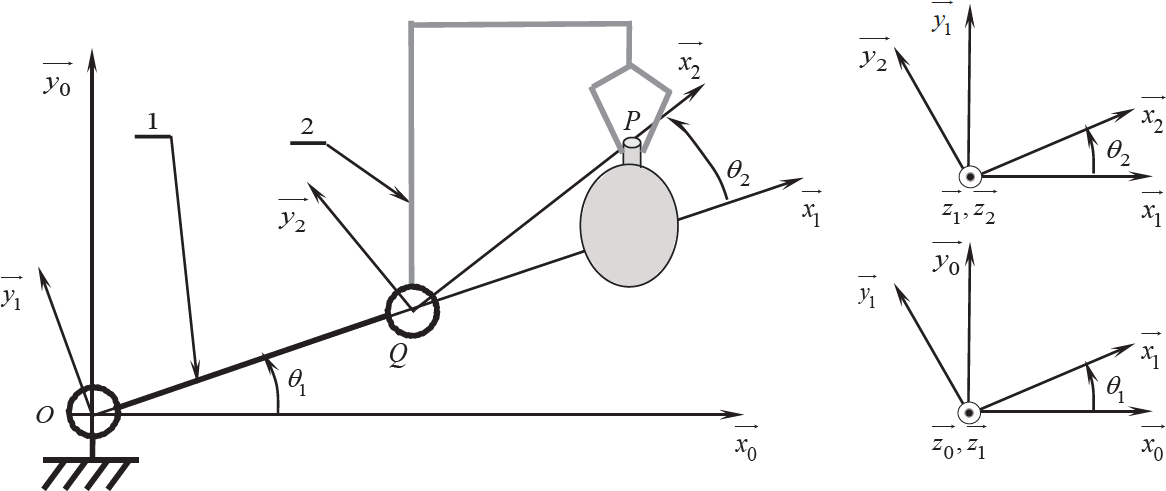
\includegraphics[width=.8\linewidth]{fig_07.png}
\caption{Schématisation cinématique du bras de déploiement \label{fig_07}}
\end{figure}




\paragraph*{Bâti 0}
Le bâti 0 est doté du repère $\rep{0} \repere{O}{x_0}{y_0}{z_0}$.

\paragraph*{Bras 1}

Le bras 1 est doté du repère $\rep{1} \repere{O}{x_1}{y_1}{z_1}$. Le mouvement de 1 par rapport à 0 est une rotation d'axe $\axe{O}{z_0}$  et d'angle $\theta_1 = \angl{x_0}{x_1}= \angl{y_0}{y_1}$. Le centre d'inertie $G_1$ est paramétré par $\vect{OG_1} = \dfrac{L}{2} \vx{1}$. De plus $\vect{OQ} = L\vx{1}$. Enfin, $m_1 = \SI{352}{g}$ et $L=\SI{0,5}{m}$.

La figure \ref{fig_08} présente le modèle volumique du bras 1. Les plans $\left(G_1,\vx{1},\vy{1}\right)$  et $\left(G_1,\vy{1},\vz{1}\right)$ sont des plans de symétrie matérielle du bras 1.

Le mouvement de 1 par rapport à 0 est commandé par un actionneur $\indice{M}{01}$, constitué d’un moteur pas à pas et d’un réducteur de vitesse à couronne dentée flexible de rapport de transmission $\lambda = 82$, d’encombrement et de masse très faibles en regard des autres solides, logés à l’intérieur de la liaison (0/1).


\paragraph*{Avant-bras 2}
L'avant-bras 2 est doté du repère $\rep{2} \repere{Q}{x_2}{y_2}{z_2}$. Le mouvement de 2 par rapport à 0 est une rotation d'axe $\axe{Q}{z_1}$  et d'angle $\theta_2 = \angl{x_1}{x_2}= \angl{y_1}{y_2}$. Le centre d'inertie $G_2$ est paramétré par $\vect{OG_2} = \dfrac{L}{2} \vx{2}$. De plus $\vect{QP} = L\vx{2}$. Enfin, $m_2 = \SI{352}{g}$ et $L=\SI{0,5}{m}$.

L’extrémité en $P$ est équipée d’une pince de masse négligeable qui saisit la sphère SEIS. On note $\indice{K}{O2}$ le moment d'inertie de l'avant-bras 2 par rapport à l’axe $\axe{O}{z_0}$ dans la position la plus défavorable.  Le mouvement de 2 par rapport à 1 est commandé par un actionneur $\indice{M}{12}$, constitué d’un moteur pas à pas et d’un réducteur de vitesse à couronne dentée flexible de rapport de transmission $\lambda = 82$, d’encombrement et de masse très faibles en regard des autres solides, logés à l’intérieur de la liaison (1/2).


\paragraph*{Sphère du SEIS : S}
On considère que l’amplitude du mouvement (S/2) est très faible. La position (S/0) repérée par : $\vect{OP}= X_P(t) \vx{0} + Y_P(t) \vy{0} $. La masse $m_s = \SI{1,2}{kg}$ est considérée comme ponctuelle en son centre d’inertie $G_S$  par rapport aux autres mouvements. $G_S$  est tel que $\vect{PG_S} = -R \vy{0}$ ($R$ est une constante positive).

%On note $\indice{K}{OS}$ le moment d'inertie de la sphère $S$ par rapport à l’axe $\axe{O}{z_0}$  dans la position $\theta_1 =\theta_2 = 0$.

\begin{obj}
Déterminer le couple du moto-réducteur $\indice{M}{01}$ qui permet la manipulation de la sphère SEIS par le système de déploiement.
\end{obj}

La figure \ref{fig_07} présente la schématisation du bras de déploiement, noté $\Sigma = \{1,2,S\}$.

%Q08 
\question{Justifier que la matrice d'inertie du bras 1, en son centre d'inertie $G_1$, est de la forme $\inertie{G_1}{O_1}=\matinertie{I_1}{J_1}{K_1}{0}{0}{0}{\rep{1}}$.}

\question{Exprimer le moment d'inertie $\indice{K}{O1}$ du bras 1 au point $O$ suivant $\vect{z_0}$ en fonction des paramètres cinétiques.}

\question{Exprimer le moment d'inertie $K_{O\Sigma}$ de l'ensemble $\Sigma$ au point $O$ suivant $\vect{z_0}$ en fonction des paramètres cinétiques.}

On considère, pour la suite, que le moteur $\indice{M}{02}$ est à l’arrêt dans la position $\theta_2 = 0$ et que seul le moteur $\indice{M}{01}$ est en fonctionnement.

\question{ Pour effectuer une modélisation dynamique du système, établir l’équation donnant le couple, 
noté $\indice{C}{01}$, du moteur $\indice{M}{01}$ en fonction des paramètres cinétiques du système de déploiement.  Préciser clairement le système isolé ainsi que le principe/théorème utilisé.}


Des calculs amènent à considérer que la valeur de $K_{O\Sigma}$ est très faible et donc pratiquement 
négligeable.

\question{Donner l’expression de l’équation précédente limitée au voisinage de la position du système de 
déploiement la plus défavorable.}
